\documentclass[11pt,letterpaper]{article}

\addtolength{\oddsidemargin}{-.875in}
\addtolength{\evensidemargin}{-.875in}
\addtolength{\textwidth}{1.75in}

\addtolength{\topmargin}{-.875in}
\addtolength{\textheight}{1.75in}

\usepackage[utf8]{inputenc}
\usepackage{caption} % for table captions
\usepackage{amsmath} % for multi-line equations and piecewises
\DeclareMathOperator{\sign}{sign}
\usepackage{graphicx}
\usepackage{relsize}
\usepackage{xspace}
\usepackage{verbatim} % for block comments
\usepackage{subcaption} % for subfigures
\usepackage{enumitem} % for a) b) c) lists
\newcommand{\Cyclus}{\textsc{Cyclus}\xspace}%
\newcommand{\Cycamore}{\textsc{Cycamore}\xspace}%
\newcommand{\deploy}{\texttt{d3ploy}\xspace}%
\newcommand{\Deploy}{\texttt{D3ploy}\xspace}%
\usepackage{tabularx}
\usepackage{color}
\usepackage{multirow}
\usepackage{float}
\usepackage[acronym,toc]{glossaries}
\newacronym{ANL}{ANL}{Argonne National Laboratory}
\newacronym{B4C}{B4C}{boron carbide}
\newacronym{BC}{BC}{boundary condition}
\newacronym{BOC}{BOC}{beginning of equilibrium cycle}
\newacronym{BSD}{BSD}{Berkeley Software Distribution}
\newacronym{BWR}{BWR}{Boiling Water Reactor}
\newacronym{CAISO}{CAISO}{California ISO}
\newacronym{CEA}{CEA}{Commissariat a l'Energie Atomique}
\newacronym{CFD}{CFD}{computational fluid dynamics}
\newacronym{CO2}{CO$_2$}{carbon dioxide}
\newacronym{CR}{CR}{control rod}
\newacronym{CRP}{CRP}{Coordinated Research Project}
\newacronym{CZP}{CZP}{Cold Zero Power}
\newacronym{DCC}{DCC}{depressurized conduction cool-down}
\newacronym{DOE}{DOE}{Department of Energy}
\newacronym[\glslongpluralkey={degrees of freedom}]{DoF}{DoF}{degree of freedom}
\newacronym{EOC}{EOEC}{end of equilibrium cycle}
\newacronym{FCEV}{FCEV}{Fuel Cell Electric Vehicle}
\newacronym{FDM}{FDM}{Finite Difference Method}
\newacronym{FEM}{FEM}{Finite Element Method}
\newacronym{FVM}{FVM}{Finite Volume Method}
\newacronym{FSV}{FSV}{Fort St. Vrain}
\newacronym[\glslongpluralkey={greenhouse gases}]{GHG}{GHG}{greenhouse gas}
\newacronym{GRS}{GRS}{Gesellschaft für Anlagen und Reaktorsicherheit}
\newacronym{H2}{H$_2$}{hydrogen}
\newacronym{He}{He}{helium}
\newacronym{HFP}{HFP}{Hot Full Power}
\newacronym{HPCC}{HPCC}{high pressure conduction cool-down}
\newacronym{HTE}{HTE}{High-Temperature Electrolysis}
\newacronym{HTGR}{HTGR}{High-Temperature Gas-Cooled Reactor}
\newacronym{HTR}{HTR}{High Temperature Reactor}
\newacronym{HTTR}{HTTR}{High Temperature Test Reactor}
\newacronym{HZDR}{HZDR}{Helmholtz-Zentrum Dresden-Rossendorf}
\newacronym{IAEA}{IAEA}{International Atomic Energy Agency}
\newacronym{icap}{iCAP}{Illinois Climate Action Plan}
\newacronym{INL}{INL}{Idaho National Laboratory}
\newacronym{IPyC}{IPyC}{inner pyrolytic carbon}
\newacronym{JFNK}{JFNK}{Jacobian-Free Newton-Krylov}
\newacronym{KAERI}{KAERI}{Korea Atomic Energy Research Institute}
\newacronym{Keff}{K$_{eff}$}{multiplication factor}
\newacronym{LBP}{LBP}{Lumped Burnable Poison}
\newacronym{LGPL}{LGPL}{Lesser GNU Public License}
\newacronym{LOCA}{LOCA}{loss of coolant accident}
\newacronym{LPCC}{LPCC}{low pressure conduction cool-down}
\newacronym{LTE}{LTE}{Low-Temperature Electrolysis}
\newacronym{LWR}{LWR}{Light Water Reactor}
\newacronym{MC}{MC}{Monte Carlo}
\newacronym{MHTGR}{MHTGR}{Modular High-Temperature Gas-Cooled Reactor}
\newacronym{MOC}{MOC}{middle of equilibrium cycle}
\newacronym{MOOSE}{MOOSE}{Multi-physics Object-Oriented Simulation Environment}
\newacronym{MPI}{MPI}{Message Passing Interface}
\newacronym{MSR}{MSR}{Molten Salt Reactor}
\newacronym{MTD}{MTD}{Champaign-Urbana Mass Transit District}
\newacronym{NEA}{NEA}{Nuclear Energy Agency}
\newacronym{NEM}{NEM}{Nodal Expansion Method}
\newacronym{NGNP}{NGNP}{Next Generation Nuclear Power}
\newacronym{NRC}{NRC}{Nuclear Regulatory Commission}
\newacronym{NSC}{NSC}{Nuclear Science Committee}
\newacronym{OECD}{OECD}{Organisation for Economic Co-operation and Development}
\newacronym{OPyC}{OPyC}{outer pyrolytic carbon}
\newacronym{ORNL}{ORNL}{Oak Ridge National Laboratory}
\newacronym{OS}{OS}{Operator-Splitting}
\newacronym{PBMR}{PBMR}{Pebble Bed Modular Reactor}
\newacronym{PDE}{PDE}{Partial Differential Equation}
\newacronym{PMR}{PMR}{Prismatic Modular Reactor}
\newacronym{PV}{PV}{photovoltaics}
\newacronym{RSC}{RSC}{Reserve Shutdown Control}
\newacronym{RSD}{RSD}{Relative Standard Deviation}
\newacronym{SD}{SD}{Standard Deviation}
\newacronym{SI}{SI}{Sulfur-Iodine}
\newacronym{SiC}{SiC}{silicon carbide}
\newacronym{SMR}{SMR}{Small Modular Reactor}
\newacronym{SNU}{SNU}{Seoul National University}
\newacronym{SOEC}{SOEC}{Solid Oxide Electrolysis Cells}
\newacronym{TIP}{TIP}{transverse integration procedure}
\newacronym{TRISO}{TRISO}{Tristructural Isotropic}
\newacronym{UIUC}{UIUC}{University of Illinois at Urbana-Champaign}
\newacronym{UNIST}{UNIST}{Ulsan National Institute of Science and Technology}
\newacronym{UK}{UK}{United Kingdom}
\newacronym{UMICH}{UMICH}{University of Michigan}
\newacronym{US}{US}{United States}
\newacronym{VHTR}{VHTR}{Very High Temperature Gas Cooled Reactor}
%\newacronym{<++>}{<++>}{<++>}
%\newacronym{<++>}{<++>}{<++>}

\definecolor{bg}{rgb}{0.95,0.95,0.95}
\newcolumntype{b}{X}
\newcolumntype{f}{>{\hsize=.15\hsize}X}
\newcolumntype{s}{>{\hsize=.5\hsize}X}
\newcolumntype{m}{>{\hsize=.75\hsize}X}
\newcolumntype{r}{>{\hsize=1.1\hsize}X}
\usepackage{titling}
\usepackage[hang,flushmargin]{footmisc}
\renewcommand*\footnoterule{}
\usepackage{tikz}
\usepackage{array}
\usepackage{booktabs,mathptmx,siunitx}
\sisetup{input-symbols = {()},  % do not treat "(" and ")" in any special way
         group-digits  = false} % no grouping of digits

\usetikzlibrary{shapes.geometric,arrows}
\tikzstyle{process} = [rectangle, rounded corners,
minimum width=1cm, minimum height=1cm,text centered, draw=black,
fill=blue!30]
\tikzstyle{arrow} = [thick,->,>=stealth]

\graphicspath{}

\begin{document}

% --------- INTRO
% \section{Introduction}

\section{The \glspl{PMR}}

% History
The history of prismatic \glspl{HTGR} or simply \glspl{PMR} begins in the 1960s with the deployment of the Dragon reactor in the \gls{UK}.
Its initial objective was to demonstrate the feasibility of the \gls{HTGR} and to launch the development of the technology.
The Dragon eeactor experiment first operated in July 1965 and reached full power of 20 MWt in April 1966.
The reactor operated for long periods at full power, demonstrated the successful operation of many components, and provided information on fuel and material irradiation tests.
Simultaneously, interest in the \gls{US} led to the 40 MWe \gls{HTGR} at Peach Bottom.
The reactor achieved initial criticality on March 1966 and went into commercial operation in June 1967.
Peach Bottom provided a valuable demonstration of the \gls{HTGR} concept by confirming the core physics calculations, verifying the design analysis methods, and providing a data base for further design activities.
Most importantly, the plant demonstrated the ability of \glspl{HTGR} to function in a load-following manner \cite{brey_development_2001}.
After the deployment of these two prototype reactors came the first \gls{HTGR} demonstration plant, the \gls{FSV} Generating Station.
Its electric power generation started in December 1976, reaching full-power operation in November 1981.
The \gls{FSV} plant generated 842 MWt to achieve a net output of 330 MWe.
This reactor laid the foundation for future \gls{PMR} designs.
Beginning with \gls{FSV}, the \gls{US} core design included ceramic coated \gls{TRISO} particles embedded within rods placed in large hexagonal shaped graphite elements \cite{brey_development_2001}.
% Despite these plants did not demonstrate the commercial capabilities of the \glspl{PMR}, they were  valuable in demonstrating attributes as the performance of the \gls{TRISO} fuel particles \cite{herranz_power_2009}.

% Safety characteristics of HTGRs
The most fundamental characteristic of the \gls{PMR} is the unique safety philosophy embodied in its design \cite{iaea_current_2001}.
The control of radionuclides does not rely on active systems or operator actions.
\gls{TRISO} particles, Figure \ref{fig:triso}, play a big role in this task.
They consist of various layers acting in concert to provide a containment structure that limits radioactive product release.
A \gls{TRISO} particle is a microsphere of about 0.8 mm diameter.
It includes a fuel kernel surrounded by a porous carbon layer (or buffer), followed successively by an \gls{IPyC} layer, a \gls{SiC} layer, and an \gls{OPyC} layer.
An additional advantage of the \gls{TRISO} particles is that they increase the proliferation resistance of \glspl{HTGR}.
They are a very unattractive and the least desirable route for diversion or theft of weapons-usable materials \cite{huning_steady_2014}.
% The buffer layer allows for limited kernel migration and provides some retention of gas compounds \cite{oecd_nea_benchmark_2017}.
% The \gls{IPyC} layer protects the kernel from chloride during the \gls{SiC} decomposition and contributes to fission gas retention \cite{demkowickz_paul_triso_2019}.
% The \gls{SiC} layer ensures the structural integrity of the particle under constant pressure and helps retain non-gaseous fission products.
% The \gls{OPyC} layer contributes to fission gas retention and protects the \gls{SiC} layer during handling.

\begin{figure}[htbp!]
	\centering
	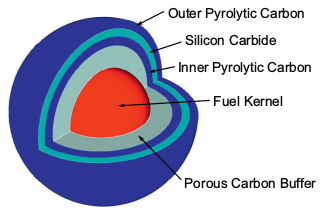
\includegraphics[height=3.5cm]{figures/triso}
	\caption{Drawing of a TRISO fuel particle. Image reproduced from \cite{hales_multidimensional_2013}.}
	\label{fig:triso}
\end{figure}

Another contributor to the passive safety of the \gls{HTGR} design is its materials.
The combination of a graphite core structure, ceramic fuel, and inert helium permits very high operating temperatures \cite{ballinger_balance_2004}.
Graphite has a high heat capacity and maintains its strength at temperatures beyond 2760 $^{\circ}$C.
As a result, temperature changes in the core occur very slowly and without damage to the core structure during transients.
Besides, the annular core geometry and a low core power density enable passive heat transfer mechanisms to remove the decay heat following postulated accidents \cite{neylan_modular_1988}.
These passive heat transfer mechanisms rely primarily on the natural processes of conduction, thermal radiation, and convection.

% Co-generation applications
A desirable feature of the \gls{HTGR} is its higher operating temperature.
Higher temperatures offer increased cycle efficiencies.
The early \gls{HTGR} designs converted their heat into electricity using the Rankine steam cycle \cite{herranz_power_2009}.
In such system, the helium coolant passes through a heat exchanger generating steam to drive a  turbine.
This arrangement is around 38\% efficient \cite{breeze_nuclear_2014}.
Some of these designs would superheat the steam to increase their efficiency, but this complicates the plant layout \cite{ballinger_balance_2004}.
A practical temperature limit is around 300-400 $^{\circ}$C.
To take advantage of the high core outlet temperature of the \gls{HTGR}, the Brayton cycle is a better option, where the helium coolant directly drives a gas turbine in a closed cycle.
With such configuration, the system can achieve an energy conversion efficiency of around 48\% \cite{breeze_nuclear_2014}.
Additionally, having helium circulating in a closed cycle removes external sources of contamination of the nuclear circuit.
Thus, the need for on-line clean up systems is largely reduced \cite{iaea_current_2001}.

Another advantage of the \gls{HTGR} over other reactor designs is that higher outlet temperatures and increased cycle efficiencies enable a wide range of process heat applications.
Some applications use steam for coal gasification processes, oil refinery processes, and  production of synthesis gas, methanol, and hydrogen.
Several hydrogen production processes benefit from high temperatures, such as high temperature electrolysis or the thermochemical splitting of water.
Utilizing the \gls{HTGR} as the energy source of the process eliminates the need to burn fossil fuels to generate the steam \cite{iaea_current_2001}.

% Maybe this paragraph should be in objectives
This thesis focuses primarily on the \gls{MHTGR}-350 \cite{neylan_modular_1988} \cite{silady_licensing_1988}.
Under the sponsorship of the \gls{US} \gls{DOE}, a team consisting of General Atomics, Combustion Engineering, General Electric, Bechtel National, Stone \& Webster Engineering, and \gls{ORNL} developed the \gls{MHTGR} \cite{neylan_modular_1988}.
They designed the basic module to deliver superheated steam at 17.3 MPa and 538 $^{\circ}$C.
Based on both economical and technological considerations, a 350 MW(t) modular reactor defines the optimal configuration.
The team completed in 1986 the preliminary safety information document for the \gls{MHTGR} and the complete draft pre-application in 1989 \cite{huning_steady_2014}.

\section{\gls{MHTGR}-350 Reactor Description}

This section provides a description of the \gls{MHTGR}-350 reactor.
Table \ref{tab:maincharac} lists its main characteristics.
The core consists of an array of hexagonal fuel elements in a cylindrical arrangement, Figure \ref{fig:layout}.
Nineteen graphite replaceable reflector elements compose the inner reflector region.
A ring of identically sized graphite replaceable reflector elements surrounds the fuel elements.
Then, a region of permanent reflector elements follows the replaceable reflectors.
The reactor vessel encases all the elements.

\begin{table}[htbp!]
	\centering
    \caption{MHTGR350 Characteristics \cite{oecd_nea_benchmark_2017}.}
	\begin{tabular}{ll}
  \toprule
	Characteristics                   & Value               \\ \midrule
	Installed Thermal Capacity        & 350 MWt             \\
	Installed Electric Capacity       & 165 MWe             \\
	Core inlet/outlet Temperature     & 259/687$^{\circ}$C  \\
	Power Density                     & 5.9 MW/m$^3$        \\
  Reactor Vessel Outside diam.      & 6.8 m               \\
	Reactor Vessel Height             & 22 m                \\
	Active core radius                & 2.97 m              \\
	Active core height                & 7.93 m              \\
  Top reflector height              & 1.20 m              \\
  Bottom reflector height           & 1.60 m              \\
	Number of fuel columns            & 66                  \\
	Number of inner reflector columns & 19                  \\
	Number of outer reflector columns & 78                  \\
  \bottomrule
	\end{tabular}
  \label{tab:maincharac}
\end{table}

\begin{figure}[htbp!]
	\centering
	\begin{subfigure}[t]{0.4\textwidth}
		\centering
		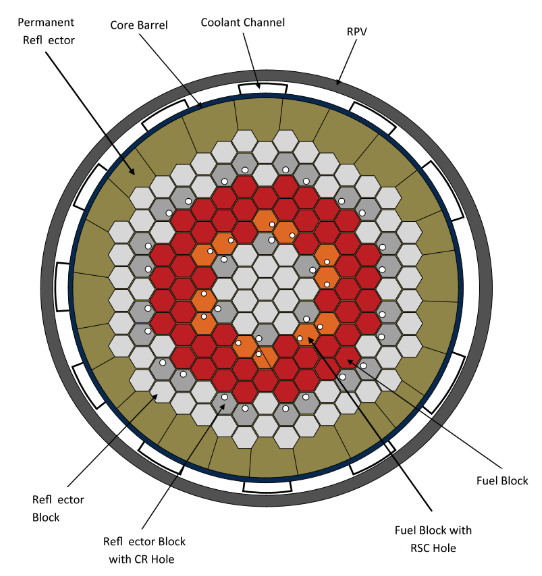
\includegraphics[width=0.95\linewidth]{figures/radial-layout.png}
		\caption{Core radial layout. Image reproduced from \cite{oecd_nea_benchmark_2017}.}
	\end{subfigure}
	\begin{subfigure}[t]{0.4\textwidth}
		\centering
		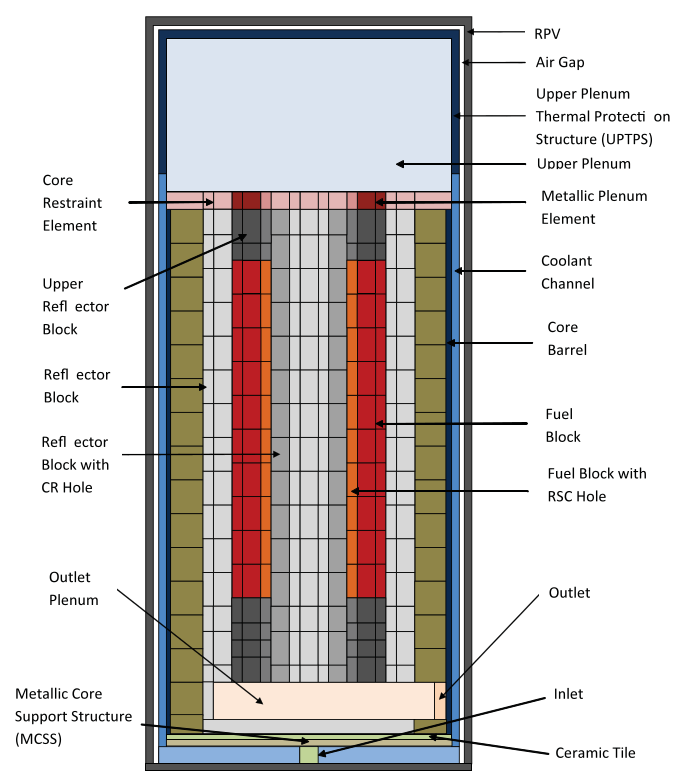
\includegraphics[width=0.95\linewidth]{figures/axial-layout.png}
		\caption{Core axial layout. Image reproduced from \cite{oecd_nea_benchmark_2017}.}
		\label{fig:layoutb}
	\end{subfigure}
	\hfill
	\caption{MHTGR reactor layout.}
	\label{fig:layout}
\end{figure}

Ten layers of fuel elements stacked on top of each other compose the 66 fuel columns that integrate the active core.
Figure \ref{fig:layoutb} shows an axial view of the reactor.
The core has two types of fuel elements: a standard element, and a reserve shutdown element that contains a channel for \gls{RSC}.
Table \ref{tab:element-characteristics} specifies the details of the MHTGR-350 fuel elements.
Twelve columns in the core contain \gls{RSC} channels for reserve shutdown borated graphite pellets.
Hoppers above the core house the pellets, and if the \glspl{CR} become inoperable, the pellets drop into the channels \cite{oecd_nea_benchmark_2017}.

\begin{table}[htbp!]
\centering
			\caption{MHTGR350 fuel element characteristics \cite{oecd_nea_benchmark_2017}.}
			\label{tab:element-characteristics}
		\begin{tabular}{@{}l S[table-format=2.2] c}
		\toprule
		\multicolumn{1}{c}{Shared characteristics} & \multicolumn{1}{c@{}}{Value} & \multicolumn{1}{c@{}}{Units} \\
		\midrule
	Block pitch (flat-to-flat)       & 36 		 & cm       \\
	Fuel length                      & 79.3 	 & cm       \\
	Fuel handling diameter           & 3.5 		 & cm       \\
	Fuel handling length             & 26.4 	 & cm       \\
	RSC hole diameter                & 9.525 	 & cm       \\
	RSC center to assembly center    & 9.756 	 & cm       \\
	Fuel/coolant pitch               & 1.879 	 & cm       \\
	Fuel hole radius                 & 0.635 	 & cm       \\
	Compacts per fuel hole           & \multicolumn{1}{c@{}}{15}   	& -        \\
	Large coolant hole radius        & 0.794 	 & cm       \\
	Small coolant hole radius        & 0.635 	 & cm       \\
  LBP hole radius                  & 0.635 	 & cm       \\
	Block graphite density           & 1.85    & g/cm$^3$ \\
	\midrule

			\multicolumn{1}{c}{Standard element} &  &  \\

	\midrule
	Number of large coolant holes    & \multicolumn{1}{c@{}}{120}   & -        \\
	Number of small coolant holes    & \multicolumn{1}{c@{}}{6}   	& -        \\
	Number of fuel holes             & \multicolumn{1}{c@{}}{210}  	& -        \\
	\midrule

			\multicolumn{1}{c}{RSC element} &  &  \\

	\midrule
	Number of large coolant holes    & \multicolumn{1}{c@{}}{88}    & -        \\
	Number of small coolant holes    & \multicolumn{1}{c@{}}{7}   	& -        \\
	Number of fuel holes             & \multicolumn{1}{c@{}}{186}  	& -        \\
		\bottomrule
		\end{tabular}
\end{table}

% Fuel assemblys and triso particles
The fuel elements contain blind holes for fuel compacts and full-length channels for helium coolant flow.
Table \ref{tab:compact} specifies details of the TRISO particle and fuel compact designs of the \gls{MHTGR}-350.

\begin{table}[htbp!]
\centering
		\caption{TRISO and fuel compact characteristics \cite{oecd_nea_benchmark_2017}.}
		\label{tab:compact}
		\begin{tabular}{@{}l S[table-format=2.1] c}
		\toprule
		\multicolumn{1}{c}{Characteristic} & \multicolumn{1}{c@{}}{Value} & \multicolumn{1}{c@{}}{Units} \\
		\midrule
	Fuel                             & UC$_{0.5}$O$_{1.5}$   & -        \\
	Enrichment (average)             & 15.5                  & wt\%     \\
	Packing fraction (average)       & 0.35                  & -        \\
	Kernel radius                    & 0.02125               & cm       \\
	Buffer radius                    & 0.03125               & cm       \\
	IPyC radius                      & 0.03475               & cm       \\
	SiC radius                       & 0.03825               & cm       \\
	OPyC radius                      & 0.04225               & cm       \\
	Compact radius                   & 0.6225                & cm       \\
	Compact gap radius               & 0.6350                & cm       \\
	Compact length                   & 4.9280                & cm       \\
	Kernel density                   & 10.50                 & g/cm$^3$ \\
	Buffer density                   & 1.00                  & g/cm$^3$ \\
	IPyC density                     & 1.90                  & g/cm$^3$ \\
	SiC density                      & 3.20                  & g/cm$^3$ \\
	OPyC density                     & 1.90                  & g/cm$^3$ \\
  Compact matrix density           & 1.74                  & g/cm$^3$ \\
	  \bottomrule
		\end{tabular}
\end{table}

% Reactivity control
A combination of \gls{LBP} and \glspl{CR} controls the core reactivity.
The \gls{LBP} consists of \gls{B4C} granules dispersed in graphite compacts.
The current design uses six \gls{LBP} rods per element.
Table \ref{tab:LBP} displays the characteristics of the \gls{LBP} compacts.

The reactor counts with 30 \glspl{CR}.
Six of them are start-up \glspl{CR} and their location is the inner reflector.
The remaining 24 are operating \glspl{CR} and control the reactivity during power operation and in case of a reactor trip.

\begin{table}[htbp!]
\centering
		\caption{\gls{LBP} compact characteristics \cite{oecd_nea_benchmark_2017}.}
		\label{tab:LBP}
		\begin{tabular}{@{}l S[table-format=2.1] c}
		\toprule
		\multicolumn{1}{c}{Characteristic} & \multicolumn{1}{c@{}}{Value} & \multicolumn{1}{c@{}}{Units} \\
		\midrule
	Absorber                         & B$_{4}$C              & -         \\
  Packing fraction                 & 0.109                 & -         \\
  Kernel radius                    & 0.0100                & cm        \\
  Buffer radius                    & 0.0118                & cm        \\
  PyC radius                       & 0.0141                & cm        \\
	Compact radius                   & 0.5715                & cm        \\
	Compact gap radius               & 0.6350                & cm        \\
  Rod length                       & 72.187                & cm        \\
	Kernel density                   & 2.47                  & g/cm$^3$  \\
	Buffer density                   & 1.00                  & g/cm$^3$  \\
	PyC density                      & 1.87                  & g/cm$^3$  \\
  Compact matrix density           & 0.94                  & g/cm$^3$ \\
	  \bottomrule
		\end{tabular}
\end{table}

% \section{GT-MHR Reactor Summary}
% Should I talk about any of this reactors GT-MHR or PMR600?

\section{Motivation}

This work's ultimate goal is to support the development of \gls{HTGR} technology.
More specifically, we focus on the development of computational methods for modeling \glspl{HTGR}.
We use \textit{Moltres} as our main analysis tool.

% Why do we focus on HTGRs?
The Generation IV Roadmap project identified reactor concepts that could meet the energy demands of the future in an efficient, economic, and environmentally safe manner \cite{macdonald_ngnp_2003}.
One of these reactor concepts is the \gls{VHTR}.
\gls{VHTR} is distinct from \gls{HTGR} as its coolant outlet temperature reaches higher temperatures.
However, the literature often uses these terms interchangeably.
In this work, the term \gls{HTGR} encompasses both terms.
The \gls{DOE} had selected this reactor concept for the, now canceled, \gls{NGNP} Project.
This project intended to demonstrate emissions-free nuclear-assisted electricity and hydrogen production by 2015.

Although the \gls{DOE} has canceled the \gls{NGNP} Project, \glspl{HTGR} will become a reality in the near future.
Some microreactor designs embody this type technology and may be operational before 2030.
Additionally, as the introduction has already described, the \gls{HTGR} technology has several favorable characteristics.
To recapitulate the most important features, the \gls{HTGR} relies on passive heat transfer mechanisms, uses TRISO particles as its fuel, has a high proliferation resistance, has the ability to achieve high temperatures, and benefits from increased cycle efficiencies.
Other beneficial characteristics are that high temperatures enable a wide range of process heat applications, among which we find hydrogen production.

%Why is computational modeling important?
Modeling and prediction of core thermal-hydraulic behavior is necessary for assessing the safety characteristics of a reactor.
Determining the temperature inside a reactor, for both normal and transient operation, is of paramount importance as the integrity of several materials depends on it.
Most importantly, undesirably high temperatures endanger the integrity of the TRISO particles and, consequently, jeopardize a fission product release \cite{tak_numerical_2008}.
% The temperatures in the core have to be kept below values that begin to cause damage to fission product barriers, produce stmctural material weakness, and lead to excessive chemical reaction rates.
Furthermore, the complex geometry of the fuel blocks hinders accurate evaluations of the fuel temperatures requiring elaborate numerical calculations.

The characteristics of a \gls{HTGR} are different from those of conventional \glspl{LWR}.
Such differences create a demand for new reactor analysis tools.
This new tools should take into account the following peculiarities of \glspl{HTGR} \cite{rohde_development_2012}\cite{bostelmann_criticality_2016}:
\begin{itemize}
\item Hexagonal structure: the shape of the fuel blocks does not conform to any orthogonal coordinate system.
\item Double heterogeneity: the TRISO particles form the first level of heterogeneity, as they consist of four layers. The second level arises from the fuel elements, as they encompass the compacts, the coolant, and the moderator.
\item Strong dependence of the neutron spectrum and the macroscopic cross sections on the fuel temperatures.
\item Long transients caused by high thermal inertia of the reactor core due to the presence of large graphite structures.
\end{itemize}

%Why use Moltres?
Historically, linking a stand-alone neutronics solver to a thermal-hydraulics solver allowed for the simulation of an entire reactor.
The coupling of the codes occurred in a black-box fashion, where the output of one code served as the input of the other, and vice versa.
This coupling technique is commonly known as the operator-splitting technique.
In such approach, each individual physics isolates the action of the governing equations upon the variables.
Nonetheless, these physical models, in reality, describe processes that rely heavily on the
solution of one another’s.
The power distribution has a strong influence on the temperature field.
Due to the \gls{HTGR} strong temperature feedback, the other way around is true as well, the temperature affects the power distribution in the core.
Because of a large time-scale separation between the different phenomena, multiphysics transient simulations coupled via the operator-splitting approach may introduce significant numerical errors  \cite{ragusa_consistent_2009} \cite{park_tightly_2010}.

\gls{MOOSE} \cite{gaston_moose_2009} is a computational framework targeted at solving fully coupled systems.
All the software built on the \gls{MOOSE} framework shares a common code base.
These feature facilitates relatively easy coupling between different phenomena and allows for great flexibility even with large variance in time scales \cite{novak_pronghorn_2018}.
Additionally, all codes use MPI for parallel communication and allow for deployment on massively-parallel cluster-computing platforms.
\textit{Moltres} \cite{lindsay_introduction_2018} is a \gls{FEM} simulation code built within the \gls{MOOSE} framework.
\textit{Moltres} solves arbitrary-group neutron diffusion, precursor, and temperature governing equations.
Besides, this simulation tool is open source.
All these characteristics make \textit{Moltres} suitable for solving the type of physical phenomena describe above.

\section{Objectives}
% This will be filled out later I guess

This thesis focuses on steady-state calculations and also intends to set a roadmap for the transient simulations.

Finally, we will compare the results to the already published results from the benchmark.

\pagebreak
\bibliographystyle{plain}
\bibliography{bibliography}

\end{document}

	% \begin{figure}[htbp!]
	% 	\centering
	% 	\begin{subfigure}[t]{0.4\textwidth}
	% 		\centering
	% 		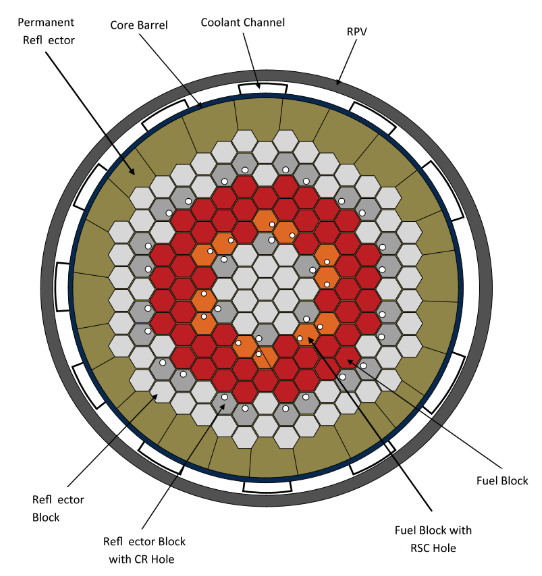
\includegraphics[width=\linewidth]{figures/radial-layout.png}
	% 		\caption{XY-plane.}
	% 	\end{subfigure}
	% 	\begin{subfigure}[t]{0.4\textwidth}
	% 		\centering
	% 		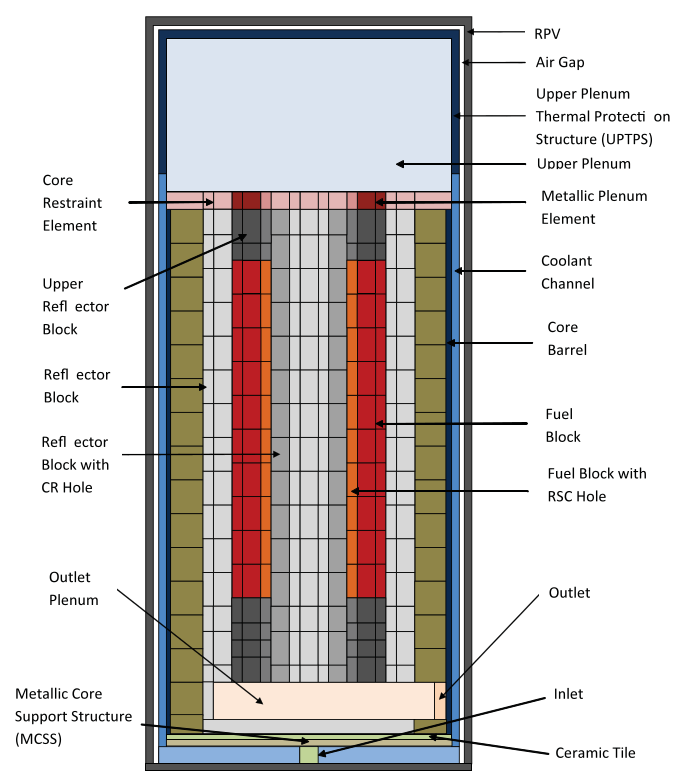
\includegraphics[width=\linewidth]{figures/axial-layout.png}
	% 		\caption{YZ-plane.}
	% 	\end{subfigure}
	% 	\hfill
	% 	\caption{MHTGR reactor layout.}
	% 	\label{fig:layout}
	% \end{figure}

	% \begin{figure}[htbp!]
	% 	\centering
	% 	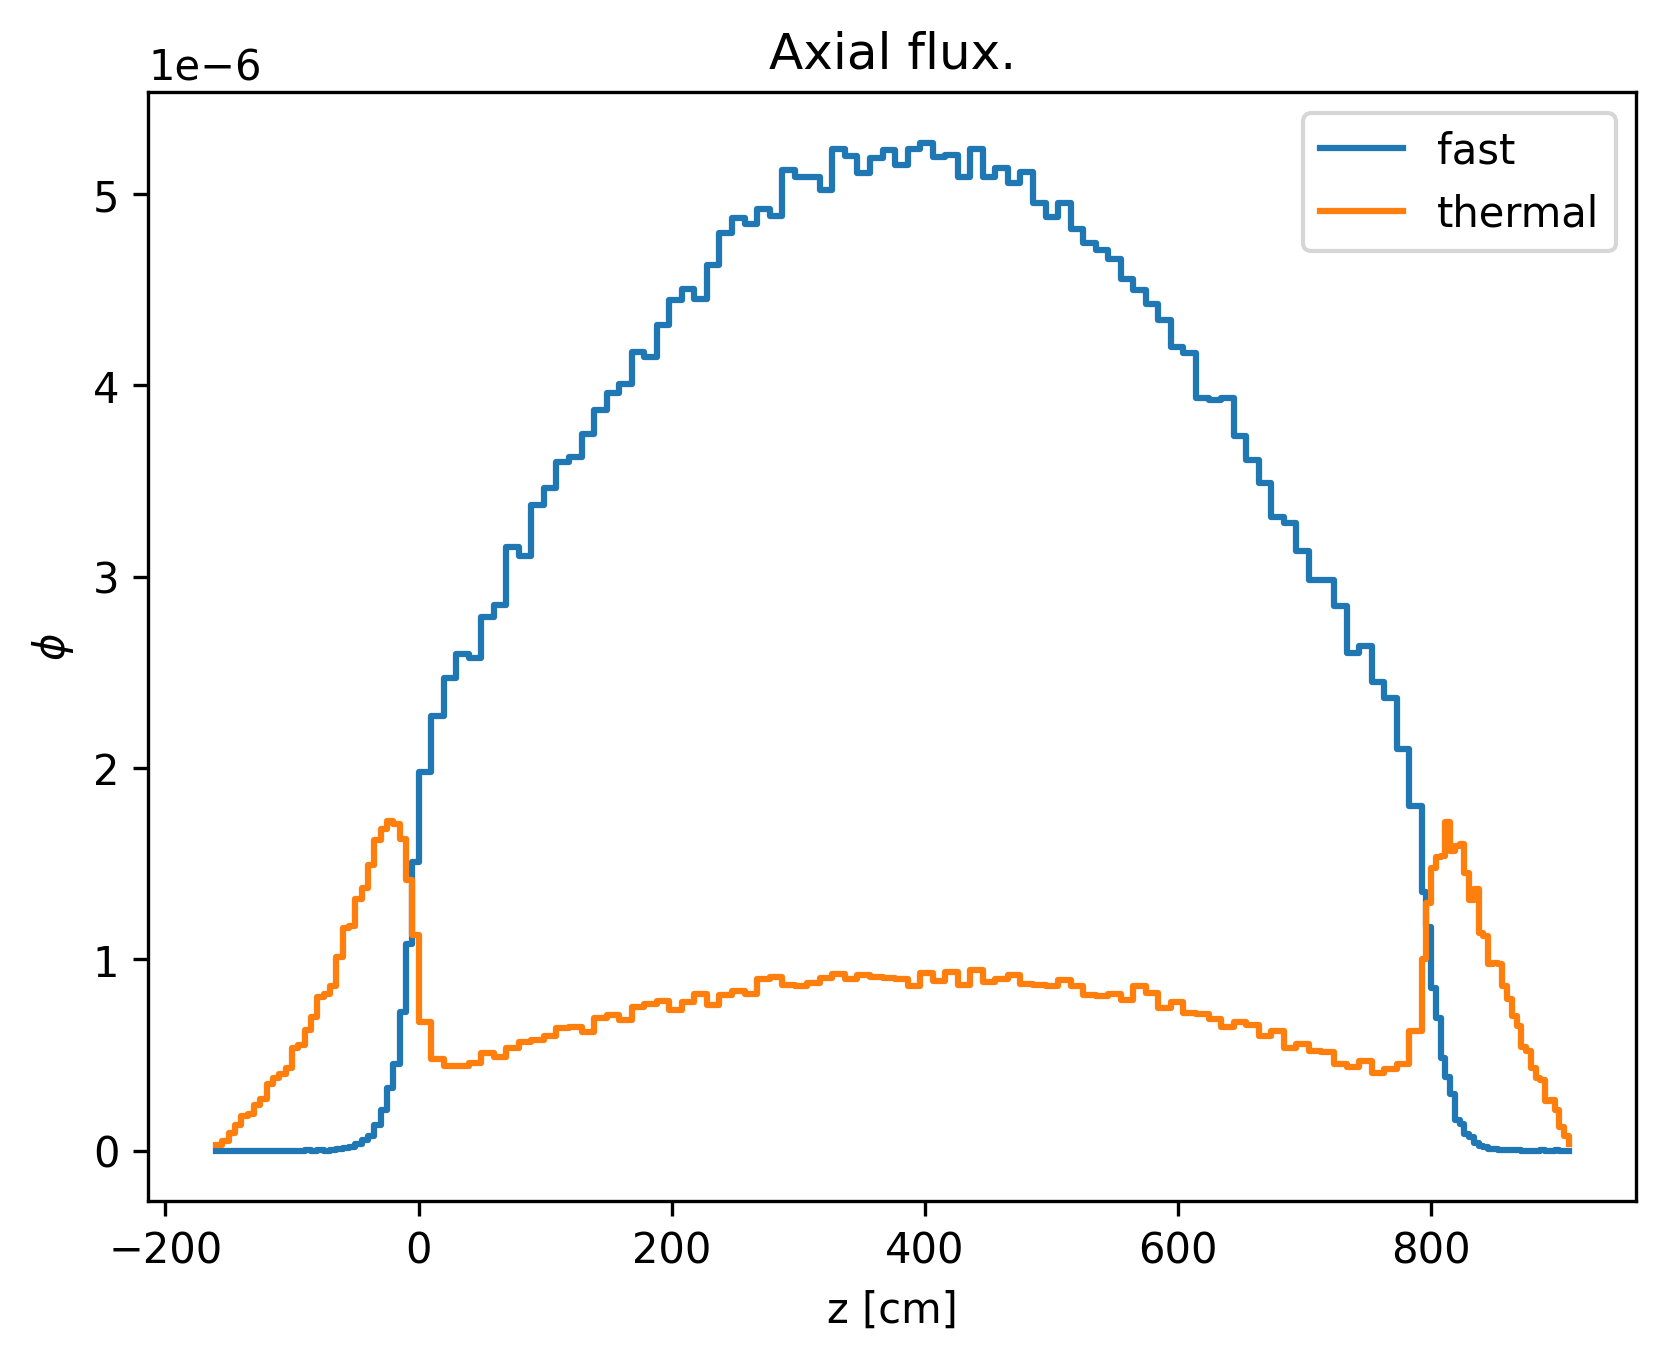
\includegraphics[width=0.6\linewidth]{figures/axial1.png}
	% 	\hfill
	% 	\caption{Neutron flux on the specified fuel channel.}
	% 	\label{fig:axial}
	% \end{figure}
